\documentclass{article}
\usepackage[utf8]{inputenc}

\title{TESS Monotransits MNRAS}
\author{Hugh Osborn}
\date{May 2020}

\usepackage{natbib}
\usepackage{graphicx}

\begin{document}

\maketitle

\section{Introduction}


\section{Analysis}

\subsection{Source of single transit candidates}
Kepler - Wang et al (Planet Huntrs), Dan Foreman Mackey, Uehara,

K2 - Osborn, LaCourse
Vanderberg (K2-2b, HIP41378), Crossfield (outer planet), Santerne (K2-239 outer planet)

TESS - Villenueva (in prep)

Also: Martti

\subsection{Stellar Parameters}\label{stellarparams}

\subsection{Monotransit search}

Given the number of monotransit candidates, and their various statuses from confirmed planet to instrumental false positive, it was necessary to create an automated vetting procedure to make sure only bona fide planet candidates are presented in this catalogue.
Similarly, because monotransits may have been initially detected in a single transit, but have later transited again, or because additional monotransiting planets may also be in the lightcurve, using the identified ephemerides was not enough, and a search for monotransits needed to be implemented.
Also, when modelling a system, the presence of other planets can both help constrain the density (through transit duration), and the eccentricity (through the prior knowledge that multiplanet systems have low-eccentricity).
Therefore any automated vetting and modelling program must also identify and model multitransiting inner planets.

In this case, the model was implemented in the following way - first signals from mono- and multi-transiting planets were searched for, then these were vetting using a variety of tests, and finally the system was modelled.

The iterative search process involved first creating reference transit models to iterate across the lightcurve.
Five models were created with \texttt{exoplanet} using the associated stellar parameters and a default radius ratio of 0.1.
As input periods, we used values between 0.4 and 2.5 times the duration of continuous observations (in the case of lightcurves with gaps longer than 5 days, the longest individual region was used).
Impact parameters were created such that they increased the gradient in duration, with the longest-duration transit (with $P=2.5P_{\rm mono}$) given $b=0.0$ and the successively shorter durations given steps up to $b=0.85$.
The five transit models, each with 500 in-transit steps yet with exposure times fixed to that of the lightcurve, were then interpolated.
This interpolated transit function formed the model to minimize at each step in the lightcurve.

Each duration was then iterated over the lightcurve, with shifts of 5\% of the transit duration each time.
At each position, three models are computed using a region 7 transit durations long around the time. The first is the interpolated transit shape with varying depth (reparameterised to $\log{\rm depth}$ to avoid negative depths) plus a gradient in the out-of-transit flux. The second is a simple 3rd degree polynomial. The third is a wavelet model with the following equation, designed to match dips due to stellar variability:
\begin{equation}
t' = 2\pi x / (2 t_D);  
F = {a}(\exp{((-t'^2) / (2\pi^2))}\sin{(t'-\pi/2)})
\end{equation}
%F = {a}(\exp{((-t'^2) / (2\pi^2))}(\sin{(t'-\pi/2)}-0.1))
Here, $t_D$ is the transit duration (set, in our case, from the interpolated transit models), and $a$ is the depth. As with the transit, a gradient was also included to account for any non-linear out-of-eclipse flux trend. 
%The shift of 0.1 is included to depress the median flux below 0.0, which is the case for dips which mimic a transit.
For each model, a likelihood is calculated and the function minimised. Bayesian Information Criterion and likelihood ratios are then calculated between each false positive model and the transit model. A transit SNR is also calculated assuming white noise.

Once every iteration, over each duration, has been computed significant detections - those where the log likelihood ratio between the transit and the other models is >4.5, and the transit has SNR>6.
The minimum DeltaBIC with respect to the polynomial model is used to choose the best transit model, and all nearby detections within $0.66t_D$ of this candidate are removed to avoid double counting.
This it iterated until no detections are classed as significant, or 8 high-SNR transit have been found.

To search for periodic transits, we first flatten the lightcurve. 
This is performed by iteratively fitting polynomials to lightcurve while also iteratively removing anomalies, as was adapted from Armstrong et al 2014.
For each small step along the lightcurve, a wide window around (but not including) each step is used to fit a polynomial.
Points in this window that had already been identified as either outliers (i.e. from detrending) or within detected monotransits (from the Monotransit search), were excluded from the polynomial fitting.
A log likelihood is computed on each of ten iterated polynomial fits, and each time a new pseudo-random mask is generated by excluding points whose scaled residual to the model is greater than a randomly-generated absolute normal distribution with unit standard deviation (thereby excluding large-residual points on the whole).
This best-fit polynomial, optimised using the wide-masked window, is then removed from the small central step to ensure any transits within are not 
For Periodic Planet searches, we used a window with duration 11 times the likely maximum duration and a stepsize of 0.1 days to ensure transits do not influence the polynomial fit.
A maximum duration is calculated assuming a circular orbit and a period of half the total observed duration, due to our limit of three transits for multi-transiting detection.

A three-transit limit at this stage is preferred to two for a handful reasons. Firstly, the implementation of period-epoch values in \texttt{transit least squares} means that allowing two transits also lets monotransits be detected, thereby duplicating our effort with the above search technique. 
Secondly, that multi-transit search is not strict about assigning only similar dips together and may conjoin either two monotransits, or the wrong two transits from a multi-transiting planet.
And thirdly, the individual transits of the majority of good duo-transiting planet are likely to be individually detectable on their own right, as the individual transits have SNR's only $1/\sqrt{2}$ (30\%) lower than the combination of both events.

The flattened lightcurves were then searched for multi-transiting planets using the \texttt{TLS} software.
If the highest periodogram peak in the TLS corresponds to a multi-transiting planet with a SNR higher than our threshold, it is stored as a new candidate.
To make sure that at least 3 transits were detected, we excluding any candidates where one or two individual transits dominated the combined SNR (defined by computing an expected SNR from the sum of each individual transit SNRs and assuring solid detections have ${\rm SNR}_i > 0.5 {\rm SNR}_{\rm expected}$).
In either case, if a signal with SNR higher that the threshold is found, we mask the detected transits by replacing all points associated with the transit with flux values randomly taken from the rest of the lightcurve.
The lightcurve is then re-scanned with \texttt{TLS} until no high-SNR candidates remain.

\subsection{Candidate vetting}
To build an automated vetting, the various possible false-positives were considered, and discriminating tests produced for each. Here we document each test performed.

Initially, we optimise a transit model using \texttt{exoplanet} and the region immediately around the detected transit ($<3.5t_D$). 
A Cubic polynomial is used to model out-of-transit flux trends, and the stellar parameters derived in \ref{stellarparams} are used.
In the case of a monotransit candidate, the period input is log-uniform between five times the initial duration and 3000, and a circular orbit is assumed and provides an initial period estimate.
In the case of multitransiting planet candidate, transit data is phase-folded and it is fitted as a monotransit with a normal prior on the log of the period centred on the detected value with standard deviation of 0.4. If the best-fit period of the candidate is discrepant from the candidate period by a factor of ten or more it is marked as a false positive, as highly discrepant densities are a proxy for eclipsing binaries on nearby stars with vastly different stellar densities.

Two signal-to-noise ratios are calculated - one by assuming the SNR is dominated by in-transit standard deviation (taken from the central 95\% of the transit), and one by calculating the median absolute deviation of the entire lightcurve binned to a cadence matching the transit duration (which effectively captures the red noise for the transit timescale).
These are then used as the initial discriminating statistics - are the recomputed white and red SNRs greater than our thresholds of 6.5 and 4.75 respectively.

Next we optimise a sinusoidal model to assess whether variability fits better than a transit. 
In this case, unlike the wavelet model fitted during the monotransit search, amplitude, duration, position, plus polynomial coefficients for a trend model are all allowed to vary.
Similarly, we construct and optimize a step model with the data, using two polynomials (each a quadratic to begin with) and a break point. 
This will fit better than a transit model for candidates caused by discontinuities in flux such as stellar flares, momentum dumps, or the start/end-of-orbit trends.
For both of these models, we perform seven initial models with random initial parameters and a randomly-chosen optimisation function, keeping that with the highest log likelihood. 
If no good model is found (defined as a model with a log likelihood$>-10^{9}$) within these seven fits, we increase the necessary polynomial and re-fit the models until one is.

Once well-fitted models are found, we recompute the transit log likelihood and compare log likelihoods, marking any candidate where the sinusoidal or step models greatly outperform the transit model ($\log{\left({L_{\rm FP}}/{L_{\rm trans}}\right)}>5$).

Next we fit a Gaussian model to the background flux. This is motivated by known false-positives in TESS data due to, i) an asteroid crossing the background aperture (which, due to the average background flux being subtract from the in-aperture flux, causes a dip) or ii) poor detrending of peaks in brightness due to reflected light.

We then fit the interpolated transit model to the x and y centroid arrays, optimising both an amplitude and a polynomial background trend in each direction. 
We then calculate a Delta BIC of the centroid model compared to a polynomial-only model, and mark the candidate as a false positive if the centroid model is preferred with a DeltaBIC$>10$.

Finally, we assemble a statistic for TESS data to encapsulate transit-like instrumental features in TESS lightcurves. To do this, the ephemerides of the TCEs cadences is used to compute how often each cadence is associated with a transit-like event.
Given the random nature of transits, any deviation in the fraction of cadences in a TCE must be due to non-astrophysical noise.
As this value does not correspond with any transit parameter such as depth, we simply use its SNR (computed with respect to the median and RMS scatter of the TCEs-per-cadence timeseries). For each monotransit candidate, the maximum  the epoch and duration of each potential monotransit signal, the significance of the maximum in-transit TCEs-per-cadence is computed.

\subsection{Single transit modelling}



\subsection{Duo-transit modelling}
Modelling two disparate transits with a range of potential periods is a challenging business.
In the case of two transits seen in single-sector TESS observations 2-years apart, a planet candidate has both a highly uncertain period ($20{\rm d}< P <750{\rm d}$) and yet a well-constrained array of possible periods to search ($P \in (t_{{\rm tr},2}-t_{{\rm tr},1})/\{1,2,3, \cdots, N_{\rm max}\}$).
However the typical toolkit for astronomers to sample the posterior distribution of some parameter - MCMC - cannot explore this extremely multi-modal parameter space.
Instead, a different modelling approach is needed to consider all potential period aliases.

One way is to perform marginalisation over the period parameter.
Bayesian marginalisation is typically performed by integrating over the relative posterior probabilities given one parameter.
\begin{equation}
p(\phi \mid d, M) \propto \int p(d \mid \phi, M) p (\phi \mid M) d\phi 
\end{equation}
Where $p(\phi \mid d, M)$ is the posterior probability for parameter $phi$ given the data $d$ and model $M$. $p(d \mid \phi, M)$ is the likelihood function (i.e. the probability of the data $d$ given parameter $\phi$ and the model $M$), and $p (\phi \mid M)$ is the prior probability of the parameter.
The evidence term on the denomination of the bayes rule, $p(d)$, is ignored here).

Rather than fitting for a period directly, a better method is to instead fit for the two transit centres, and marginalise over the integer number of periods between them.
This means the marginalisation becomes a sum over the product of the likelihood and prior for each period alias.
\begin{equation}
p(\phi \mid d, M) \propto \sum^{i=0}_{n_{\rm alias}} p(d \mid \phi, M) p (\phi \mid M) \;
\end{equation}

\subsubsection{The Period prior}
% # circular prior: P^(-8/3)
% # eccentric prior: P^(-2) * sep_in_transit^(-1)
% # Star-crossing prior: any orbit which crosses the stellar disc hit with -500 in logprior
% # Orbit-crossing prior: any orbit which crosses the orbit of an interior (multi) has -500 in logprior
% # p(P|b) prior which includes both dp_db component & component for unphysical durations
The correct prior for orbital period given incomplete knowledge was well explored by \citet{Kipping2018}.
This suggested that the correct prior is a combination of terms representing:
\begin{itemize}
    \item An intrinsic prior for exoplanet occurrence, $p({\rm Tr} \mid P) \propto P^\alpha$, where $\alpha=\frac{2}{3}$ represents an occurrence distribution flat in $\log{P}$.
    \item A prior from the "window effect" from the probability of observing a transit of a planet ($p({\rm Tr}$) given some period $P$ and observing window of length $W$, $p({\rm Tr} \mid W) \propto W/P$.
    \item The geometric transit probability, as planets on long orbits are less likely to transit their stars with a probability $p({\rm Tr} \mid a) = R_s/a$ which, when rearranged using Kepler's third law becomes $p({\rm Tr} \mid P) \propto P^{-2/3}$.
\end{itemize}
Resulting in a prior on orbital period of $P^{-8/3}$.

However, such a prior is only true for circular orbits, and when an eccentric orbit is considered, a prior on only period is not possible.
Instead, the geometric prior must be updated to include the planet-star separation during transit, and therefore the eccentricity $e$ and argument of periasteron $\omega$
\begin{equation}
p({\rm Tr} \mid e,a,\omega) = (R_s (1+ e\cos(\omega-\pi/2)) /(a (1-e^2)) \;
\end{equation}

Another prior can be included in the case of an eccentric orbit - the planets periasteron ($(a/R_s)*(1 - e)$) cannot intersect the star, and indeed is unlikely to pass within $2R_s$, where tidal forces would quickly recircularise the planet.
Therefore, to avoid these unphysical orbits in our model, we include a sharp prior using a sigmoid function with $mu = 2R_s$ with output values betwee -500 (for star-scraping orbits) and 0.0 (for "safe" orbits), with a width of $0.05R_s$.

In the case of multi-planet systems, we also have extra information from the presence of other planets in the system - to be stable their orbits should not cross.
Therefore we apply the same prior as above using the orbit of the outer-most "multi-transiting" planet candidate (i.e. with a certain period). 

\subsubsection{Reparameterisation}

The morphology of exoplanet transits is dominated by the transit depth and duration. 
Transits models typically explore a parameter space in impact parameter \& radius ratio  (ignoring orbital constraints \& limb darkening parameters), with the former dominating the transit depth, and a combination of $b$ and orbital motion producing the transit duration.

In the case of transits associated with mono- or duo-transiting planets, the difference between orbital velocities between samples can be an order of magnitude. 
This therefore means that impact parameter is no longer the dominant source of the impact parameter, and even more problematically, the jumps between orbital solutions (due to either gaps in the lightcurve or period aliases) mean transit duration may jump between samples, making MCMC parameter exploration difficult.

One way to avoid this problem is to re-parameterise a transit model from sampling in b to sampling directly in tdur.
The simplest reformulation uses the approximate transit duration (this requires a small-angle approximation, i.e. that the planet's transit can be approximated to a straight line) and reuires the planet-to-star radius ratio, $R_p/R_s$, the period, $P$, gravitational constant $G$, and the stellar density $\rho_s$.
\begin{equation}
T_{\rm dur, circ} = \sqrt{(1+R_p/R_s)^2 - b^2} (\frac{3 P}{\pi^2 G \rho_s})^{1/3}  \;
\end{equation}
This can then be adjusted to incorporate the change in planet velocity during transit (again, assuming the planetary transit can be approximated to a constant tangential velocity).
\begin{equation}
T_{\rm dur} = T_{\rm dur, circ} \frac{\sqrt{1-e^2}}{1+e\cos{(\omega - \pi/2)}} \;
\end{equation}
When written in terms of $b$, this becomes
\begin{equation}
b = \sqrt{(1+R_p/R_s)^2 - T^2 (\frac{1+e\cos{(\omega - \pi/2)}}{\sqrt{1-e^2}})^2 (\frac{\pi^2G\rho_s}{3P})^{2/3}} \;
\end{equation}
However transit durations do not map perfectly to impact parameter - any duration longer than the maximum (i.e. $b=0$) duration given by the other parameters does not have a real b value.
In these cases, we set impact parameter to zero and applied a strong prior to drive the MCMC chains to physical values.

One of the benefits of sampling in b is that a uniform b is akin to sampling in uniform inclinations - i.e. this should match reality and no prior is needed.
This is no longer true in the case of determining b from other parameters.
Consider a short duration transit that requires a grazing eclipse to match the period - due to the geometry of the stellar disc the duration is extremely susceptible to impact parameter, and the chord that approximates the duration is extremely small. 
To take that into account in this re-parameterisation, we apply a marginal prior to each period taken from the differential of the impact parameter with respect to the orbital period.
As period can be derived from impact parameter using the following equation


\begin{equation}
P = (\pi^2 G \rho_{\rm s} /3)(\frac{((1+R_p/R_s)^2 - b^2)(1-e^2)}{T^2 (1+e\cos{(\omega - \pi/2)})^2})^{3/2} \;
\end{equation}
\begin{equation}
p(b \mid P) = \frac{d b}{d P} \propto b^{-1}P^{-5/2} \;
\end{equation}

% \begin{equation}
% $$ p(b \mid P) \sim \frac{d b}{d t_{\rm dur}} \propto - P^{2/3} / b  \;$$
% %= -\frac{t_{\rm dur}}{b}(\frac{3P}{\pi^2 G \rho_S})^{2/3} = $$
% \end{equation}

2021 re-write

Transit duration, impact parameter and perpendicular velocity can each be derived from the other two, as the former two set the time and distance needed to calculate a velocity.
Typically, transit modelling derives a velocity from input orbital elements (e.g. orbital period, eccentricity and argument of periasteron), and therefore fits for either the duration or the impact parameter and not both.
In the case where a period is not a priori well-constrained, this leaves an open approach for which two of the three to model.
Here we show how \texttt{MonoTools} models transits by fitting for impact parameter and duration while deriving orbital velocity and orbital period.



\begin{figure}[h!]
\centering
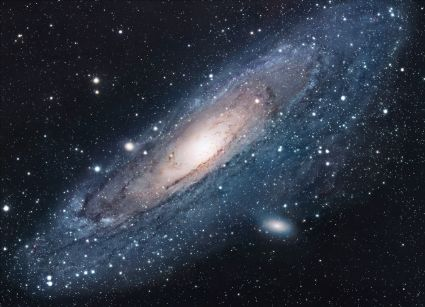
\includegraphics[scale=1.7]{universe}
\caption{The Universe}
\label{fig:universe}
\end{figure}

\section{Conclusion}
``I always thought something was fundamentally wrong with the universe'' \citep{adams1995hitchhiker}

\bibliographystyle{plain}
\bibliography{references}
\end{document}
